\documentclass[11pt,letterpaper]{article}
\usepackage[margin=0.9in]{geometry}
\usepackage[T1]{fontenc}
\usepackage{lmodern,microtype,amsmath,amssymb,booktabs,tabularx,graphicx}
\usepackage[dvipsnames]{xcolor}
\usepackage{listings,enumitem,tikz,fancyhdr,caption,float,needspace}
\usetikzlibrary{arrows.meta,positioning}
\usepackage[colorlinks=true,linkcolor=MidnightBlue,urlcolor=MidnightBlue,citecolor=MidnightBlue]{hyperref}
\definecolor{ink}{HTML}{243448}
\definecolor{accent}{HTML}{147E77}
\definecolor{codebg}{HTML}{F5F7F9}
\hypersetup{pdftitle={Above-Fundamental Trading in an EDSL Asset Market},pdfauthor={}}
\pagestyle{fancy}\fancyhf{}
\fancyhead[L]{\small EDSL asset-market pilot}
\fancyhead[R]{\small GPT-5 mini / speculative-v1}
\fancyfoot[C]{\thepage}
\setlength{\headheight}{14pt}
\setlength{\parindent}{0pt}
\setlength{\parskip}{5pt}
\setlength{\emergencystretch}{2em}
\setlist{nosep,leftmargin=*}
\captionsetup{font=small,labelfont=bf}
\lstdefinestyle{python}{language=Python,basicstyle=\ttfamily\footnotesize,
 keywordstyle=\color{MidnightBlue}\bfseries,commentstyle=\color{OliveGreen},
 stringstyle=\color{BrickRed},backgroundcolor=\color{codebg},
 breaklines=true,breakatwhitespace=false,columns=fullflexible,keepspaces=true,
 showstringspaces=false,numbers=left,numberstyle=\tiny\color{gray},
 numbersep=7pt,xleftmargin=17pt,frame=single,framerule=0pt,
 aboveskip=9pt,belowskip=9pt,tabsize=4,
 literate={–}{{\textendash}}1}
\lstset{style=python}
\newcommand{\code}[1]{\texttt{\small #1}}
\newcommand{\source}[1]{\textit{Executed source:} \path{#1}. Line numbers refer to the frozen source file.}
\newcommand{\WalkImports}{\lstinputlisting[firstline=12,lastline=33,firstnumber=12]{code/portable.py}}
\newcommand{\WalkSchema}{\lstinputlisting[firstline=36,lastline=49,firstnumber=36]{code/portable.py}}
\newcommand{\WalkPersonas}{\lstinputlisting[firstline=51,lastline=115,firstnumber=51]{code/portable.py}}
\newcommand{\WalkQuestion}{\lstinputlisting[firstline=118,lastline=160,firstnumber=118]{code/portable.py}}
\newcommand{\WalkAgents}{\lstinputlisting[firstline=163,lastline=176,firstnumber=163]{code/portable.py}}
\newcommand{\WalkMarket}{\lstinputlisting[firstline=179,lastline=201,firstnumber=179]{code/portable.py}}
\newcommand{\WalkPause}{\lstinputlisting[firstline=204,lastline=232,firstnumber=204]{code/portable.py}}
\newcommand{\WalkPlan}{\lstinputlisting[firstline=235,lastline=252,firstnumber=235]{code/portable.py}}
\newcommand{\WalkBuild}{\lstinputlisting[firstline=255,lastline=325,firstnumber=255]{code/portable.py}}


\begin{document}
\begin{center}
{\LARGE\bfseries\color{ink} Above-Fundamental Trading\\[3pt] in an EDSL Asset Market}\par
\vspace{5pt}
{\large A short GPT-5 mini pilot with behavioral trader personas}\par
{\small September 2026 \quad $\cdot$ \quad Exploratory simulation note}
\end{center}

\begin{abstract}
Twelve LLM traders interacted through a persistent, sealed-order call market.
With newly authored speculative prompts and GPT-5 mini, the first transactions
occurred in rounds 16 and 17 at \$17.53 and \$17.67, respectively, against a
constant \$14 fundamental value. Volume was 2 and 19 shares. The observation
then stopped under a two-consecutive-prices rule. This is evidence of early
above-fundamental trading in one market; the two observed price points do not
establish a full bubble-and-crash path. EDSL elicited all 204 trader decisions;
shared-state commands performed the 17 settlements deterministically.
\end{abstract}

\section{Design and observation}
The market reconstructs the economic environment in the supplied presentation
by Ngo et al.\ \cite{ngo}. Each of 12 traders starts with \$100 and four shares.
The economic horizon is 30 rounds. After trading in each round, cash earns 5\%
interest and every share pays a common dividend of \$0.40 or \$1.00, each with
probability one-half. Shares are redeemed for \$14 after round 30's income.
With $n=31-t$ remaining payments, the expected-dividend benchmark before round
$t$ is
\[
 V_t=\sum_{k=1}^{n}\frac{0.70}{1.05^k}+\frac{14}{1.05^n}=14.
\]
This is the frictionless expected-value benchmark; the implementation rounds
money to cents. Traders cannot borrow or short shares. Each submits one buy,
sell, or hold decision and forecasts for the current round and 2, 5, and 10
rounds ahead. Crossing orders clear at a single price.

The market uses seed 140926 and contains two each of Rational Arbitrageurs (RA), Momentum
Chasers (MC), Bubble Timers (BT), Precommitters (PC), Noise Traders (NT), and
Overconfident Contrarians (OC). The \code{speculative-v1} prompts encourage
resale-based beliefs, early speculative interest, and explicit exit plans.
They disclose the economic rules, including terminal redemption, but do not
supply the \$14 valuation answer or an opening market quote. These are
\emph{new exploratory prompts}, not the source authors' original prompts.
The source's highlighted theory composition is BT+OC+PC, whereas this pilot
uses all six types.

The initial observation cap was 12 rounds, with an earlier stop after two
consecutive actual prices at or above \$17.50 (25\% above fundamental). After
six rounds without trades, inspection of the PCs' stated schedules revealed
selling windows starting in rounds 16 and 26. A conditional extension to round
20 was declared if round 12 still had no trades. That condition held; the saved
market resumed and reached the price-based stop at round 17. This adaptive
extension is part of the exploratory design. The economic horizon stayed at
30 throughout: the pause did not redeem any shares.

\clearpage
\section{Prices, orders, and participation}
\begin{figure}[H]
\centering
\includegraphics[width=\linewidth]{figures/market.pdf}
\caption{Quotes rose before any trade occurred. Missing transaction prices in
rounds 1--15 are left missing. The bid and ask series summarize sealed orders
for analysis; traders did not see other traders' quotes. The \$17.50 line is the
observation stopping threshold.}
\label{fig:market}
\end{figure}

\begin{center}
\begin{tabular}{lrrr}
\toprule
Round(s) & Clearing price & Shares traded & Premium to \$14 \\
\midrule
1--15 & No transaction & 0 & --- \\
16 & \$17.53 & 2 & 25.21\% \\
17 & \$17.67 & 19 & 26.21\% \\
\bottomrule
\end{tabular}
\end{center}

There were no sell orders in the first 15 rounds. During that interval the
highest bid rose from \$15.00 to \$22.00, reaching \$22.50 in round 16.
Those bids are willingness-to-pay statements, not a transaction-price path.
Trader 09 (PC) supplied the first two shares in round 16 at a \$14.05 sell limit.
One share went to trader 00 (MC) and one to trader 02 (NT), both at \$17.53.

After that first public price, more sellers entered. In round 17 both RAs
offered their initial holdings; one sold four shares and the other sold three.
Other sellers were a PC, an NT, a BT, and an OC. Purchases were concentrated:
trader 02 (NT) bought 11 of the 19 shares, trader 10 (BT) bought six, and the two
MCs bought one each. Trader 02 ended with 16 of the market's 48 shares.
Figure~\ref{fig:decisions} shows every trader's action and actual fills.

The two clearing prices differ by only \$0.14 (0.80\%). Thus the clearest
finding is \emph{overpricing when trade begins}, preceded by rising speculative
bids. There are too few transaction-price observations to measure a sustained
inflation trajectory. Total traded volume is 21 shares; this counts turnover,
not necessarily distinct shares.

\clearpage
\begin{figure}[H]
\centering
\includegraphics[width=\linewidth]{figures/decisions.pdf}
\caption{All 204 decisions. Cell color indicates the submitted side. Numbers
are signed executed quantities: positive for purchases, negative for sales.
An unnumbered buy or sell cell had no fill. Trader IDs are shortened to their
two-digit suffixes. All orders passed validation without quantity reductions.}
\label{fig:decisions}
\end{figure}

\subsection*{How the clearing rule produced the prices}
The exchange expands admitted quantities into unit orders, sorts bids from
highest to lowest and asks from lowest to highest, and finds the largest
crossing quantity $q$. It sets one price at the midpoint of the marginal
matched bid and ask, rounded half up to cents:
\[
 q=\max\{k:b_k\geq a_k\},\qquad
 p=\operatorname{round}_{\mathrm{cent}}\!\left(\frac{b_q+a_q}{2}\right).
\]
If there is no crossing pair, the recorded price is null. The midpoint and
tie-allocation rules are reconstruction choices, and can affect measured
overpricing. In round 16, the marginal bid was \$21.00 and the ask was \$14.05:
their midpoint yields \$17.53. In round 17 the marginal pair was \$17.80 and
\$17.53, yielding \$17.67. The first price therefore did not require the seller
to demand a 25\% premium; the aggressive buy side and the midpoint rule jointly
produced it. Figure~\ref{fig:clearing} in the appendix shows both order books.



\clearpage
\section{Interpretation and implementation}
\textbf{The outcome.} This market generated two consecutive rounds of trading
more than 25\% above the expected-dividend benchmark. That is consistent with
the intended speculative treatment producing bubble-like overpricing. It is
not an estimate of bubble frequency, a demonstration of a crash, or a numerical
replication of the source study. Only one market is reported, and observation
was extended and stopped using its outcomes. No post-peak drawdown is observed.

\textbf{What the traders said.} At the opening, trader 00 (MC) correctly noted
that fundamental present value was about \$14, but bid \$15 to avoid missing a
rally. In round 16 it bid \$22.50 despite acknowledging no transaction history.
Following the first trade, the RAs described the observed \$17.53 as overpriced
and offered shares, while trader 10 (BT) bought in anticipation of resale above
\$18. These statements support a speculative-resale interpretation for some
decisions, but are model-generated explanations, not independent measurements
of latent beliefs. Errors remain: trader 00 described its round-17 bid as a
raise even though its submitted limit fell from \$22.50 to \$18.00. A more capable
model did not eliminate inconsistencies.

\textbf{Why GPT-5 mini.} Earlier selected-case comprehension checks scored
GPT-5 mini at 155/156 factual items versus 128/156 for GPT-4o-mini. GPT-5 mini
also better respected inventory in the selected trade replays. These checks
motivated the model choice; they are not a broad model benchmark or a controlled
estimate of the model's effect on bubbles. The present run used medium
reasoning, temperature 1, and an 8,000-token completion allowance, including
reasoning tokens. Raw responses identify \code{gpt-5-mini-2025-08-07}.

\textbf{What EDSL did.} Each trader's decision was elicited with an EDSL
\code{QuestionDict} survey. A private shared-state view supplied current cash,
inventory, prior decisions and fills, and the public transaction history.
All 12 round-specific questions were opened before any answers were committed.
Calls then ran concurrently; sealed submissions committed on one event loop.
A workflow dependency barrier released the deterministic exchange only after
all 12 submissions. No LLM selected clearing prices, allocated fills, or updated
balances. ``Local'' execution here means EDSL called hosted OpenAI directly;
it does not mean an on-device model. Appendix~\ref{app:workflow} details the
workflow. Subsequent appendices present a self-contained rewrite using the
new native APIs; the executed source files are preserved in the bundle.

\textbf{Execution checks.} The saved audit reconciles 204 model responses,
204 order submissions, 17 settlements, and 221 successful workflow attempts.
It checks accounts, inventory constraints, fills against limit prices, private
observations, rendered prompts, source fingerprints, and the absence of early
redemption. No orders were rejected or quantity-capped in this run. All 48
shares remained live at the pause; recorded model cost was \$0.5741. A final
Results-package export error after resumption was repaired from durable raw
responses without additional model calls or market commands
(Appendix~\ref{app:reproduce}).

\begin{thebibliography}{1}
\bibitem{ngo}
Cady Ngo, Yi-Jhe Chen, Benjamin Manning, Christopher Avery, and Colin Camerer.
\emph{Building Traders: Persona Construction for LLM Agents in Experimental
Asset Markets}. Supplied 40-page presentation, dated September 18, 2026,
file \code{140926.pdf}. Design: pp.\ 10--11; archetypes: p.\ 14;
highlighted composition: pp.\ 16, 25. This citation describes the supplied slides.
\end{thebibliography}

\clearpage
\appendix
\section{Workflow and information boundaries}\label{app:workflow}
The run uses the branch's Python workflow and shared-state APIs. The workflow
definition fixes all 30 economic rounds. The delivery loop decides how much of
that definition to execute before pausing. The native rewrite below encodes
these checkpoints as workflow pause rules. Stopping observation and terminating
the economic experiment are separate operations.

\begin{figure}[H]
\centering
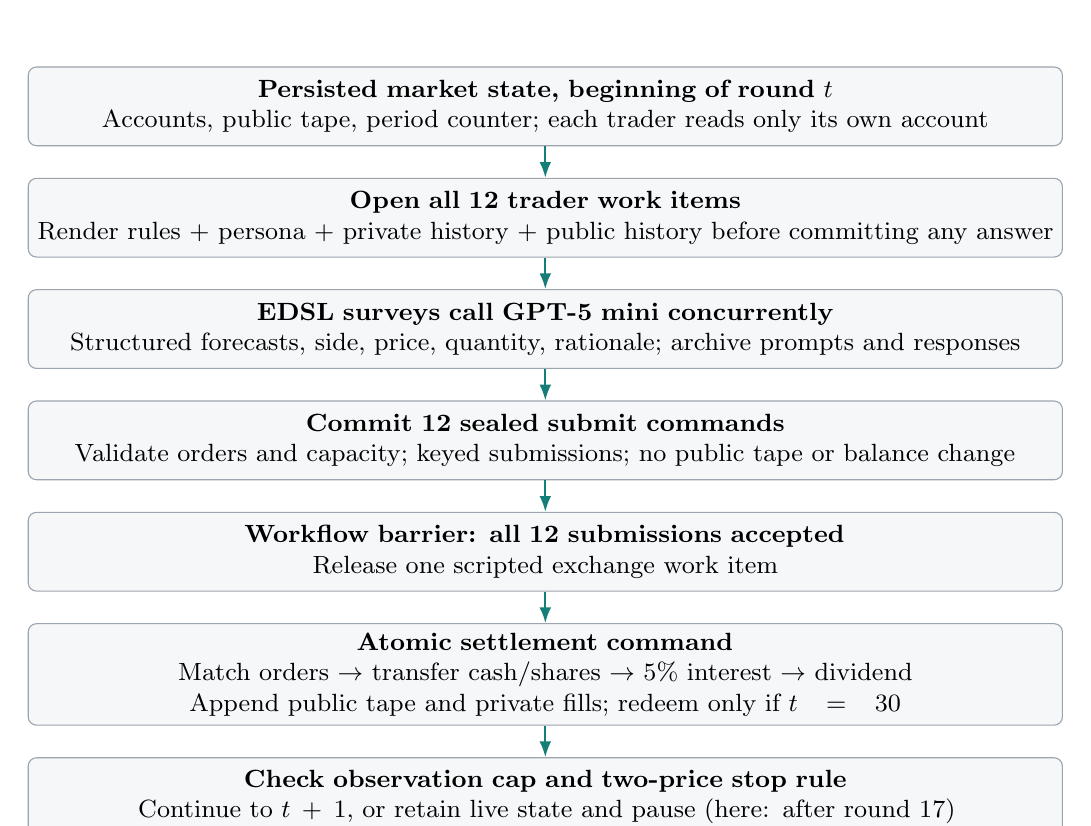
\begin{tikzpicture}[
 node distance=4mm,
 box/.style={draw=ink!45,rounded corners=3pt,fill=codebg,align=center,
 text width=12.9cm,minimum height=10mm,font=\small},
 arr/.style={-{Latex[length=2mm]},thick,draw=accent}]
\node[box] (s) {\textbf{Persisted market state, beginning of round $t$}\\
 Accounts, public tape, period counter; each trader reads only its own account};
\node[box,below=of s] (o) {\textbf{Open all 12 trader work items}\\
 Render rules + persona + private history + public history before committing any answer};
\node[box,below=of o] (l) {\textbf{EDSL surveys call GPT-5 mini concurrently}\\
 Structured forecasts, side, price, quantity, rationale; archive prompts and responses};
\node[box,below=of l] (c) {\textbf{Commit 12 sealed submit commands}\\
 Validate orders and capacity; keyed submissions; no public tape or balance change};
\node[box,below=of c] (b) {\textbf{Workflow barrier: all 12 submissions accepted}\\
 Release one scripted exchange work item};
\node[box,below=of b] (e) {\textbf{Atomic settlement command}\\
 Match orders $\to$ transfer cash/shares $\to$ 5\% interest $\to$ dividend\\
 Append public tape and private fills; redeem only if $t=30$};
\node[box,below=of e] (p) {\textbf{Check observation cap and two-price stop rule}\\
 Continue to $t+1$, or retain live state and pause (here: after round 17)};
\foreach \a/\b in {s/o,o/l,l/c,c/b,b/e,e/p}{\draw[arr] (\a)--(\b);}
\end{tikzpicture}
\caption{One round of the implemented workflow. SQLite stores both the
coordination record and the evolving market; raw EDSL results are also archived.}
\end{figure}

\subsection*{Who can observe what?}
The market state holds all accounts and sealed orders, but the trader read view
contains just the current period, public tape, its own account and history,
an internal last-price field, and a finished flag. The speculative question
template renders selected fields: it does not display sealed orders, other
accounts, the internal last-price field, or the tape's reference-price field.
Thus an initial internal value of 14 is not presented as a fabricated trade.
No-trade rounds explicitly display a null transaction price.

\subsection*{Persistence and recovery}
The workflow store records work items, delivery attempts, accepted answers,
and events; the state backend records state reads and command effects.
Each submission has a work-item-specific idempotency key. Resuming
restores the pinned workflow and recovers outstanding coordination work.
Source hashes and economic/model configuration must match before continuation.
The seed fixes seat allocation, dividends, and tie priority; it does not make
fresh hosted model responses deterministic.

\clearpage
\section{Prompts and structured EDSL questions}\label{app:prompts}
Appendices B--D walk through one self-contained file,
\path{code/portable.py}. It contains all prompts, agent construction, market
configuration, workflow dependencies, pause rules, and the execution plan.
Its imports are limited to Python's standard library and EDSL.

This rewrite uses the branch's new native \code{call\_market},
\code{WorkflowExperiment}, and \code{pause\_after} APIs. It was written after
the reported run. The four original source files remain in the bundle as the
execution record. Every trader instruction and all 30 question templates match
the historical construction. Replaying the 204 saved decisions with the native
market commands reproduces the complete accounts, orders, and transaction tape.
The authoring file also matches the saved portable specification, allowing for
fresh internal identifiers. These checks involve zero new model calls.

\subsection{Imports and the eight answer fields}
\WalkImports
\Needspace{4\baselineskip}
\par\noindent
\begin{minipage}{\linewidth}
\WalkSchema
\code{KEYS} names the eight values returned by each trader: four price
forecasts, a side, a limit price, an integer quantity, and a rationale.
\code{COMPOSITION} gives the archetypes in their pre-shuffle order.
\end{minipage}
\par

\subsection{Common objective and the six personas}
The common objective is combined with one persona in each agent's instruction.
The full instructions are reproduced here without abbreviation.
\WalkPersonas

\subsection{The question and its private-state template}
Private history includes admitted quantities and signed fills so intended
trades are distinguishable from executed trades. The template receives the
current trader's account and the public tape; forecasts do not mechanically
set execution prices.
\WalkQuestion

\subsection{Create the twelve traders and the exchange}
The six-type list is repeated twice, then shuffled using seed 140926. Each
trader gets its own name, role, seat, and full instruction. The exchange is a
separate workflow participant whose work is performed by deterministic code.
\WalkAgents

\Needspace{0.52\textheight}
\subsection*{An actual first decision}
The bundle includes \path{data/example-system-prompt.txt} and
\path{data/example-user-prompt.txt}, copied from the actual EDSL call for
\code{trader-00}, round 1. These preserve the fully rendered presentation,
including EDSL's output instructions. Its structured answer is shown below;
the rationale is the model's elicited text, not an observer's description.
The submitted buy of one share at \$15 received no fill because there were no
sell orders.
\lstinputlisting[language={},numbers=none]{data/example-answer.json}

\Needspace{0.25\textheight}
\section{Shared-state market implementation}\label{app:state}
The exchange is configured with \code{call\_market}. Its versioned commands
are provided by EDSL's standard runtime: \code{call\_market\_submit@1} and
\code{call\_market\_settle@1}. The experiment needs no custom settlement
callback or registration step. The JSON carries the economic parameters and
required capability versions; the installed EDSL runtime supplies their code.

\par\noindent
\begin{minipage}{\linewidth}
\subsection{Explicit economic configuration}
\WalkMarket
\end{minipage}
\par

Cash is stored in integer cents. The income list is ordered: 5\% interest
on post-trade cash, then a common dividend. The internal reference price does
not appear in the question as a market quote. Redemption occurs only after
round 30's income, even when observation pauses sooner.

\subsection{Admission and clearing semantics}
Forecasts must be finite and nonnegative. The exchange validates side, price,
and quantity; caps buys by available cash divided by the limit and by 48 shares;
and caps sells by inventory. Invalid order fields receive zero admitted
quantity with a rejection recorded; bad forecasts raise an exception.
Duplicate and stale submissions are refused. Submission changes neither
balances nor the public tape. All orders in this run were admitted unchanged.

Settlement requires all 12 submissions. Unit bids descend, unit asks ascend,
and crossing units trade at one price: the midpoint of the marginal matched
bid and ask, rounded half up to cents. Equal-price priority follows a seeded
lottery independent of answer arrival. Trading conserves cash and shares;
interest and dividends are added afterward. Unfilled orders expire. A round
without crossing orders records zero volume and a null transaction price.

\begin{figure}[H]
\centering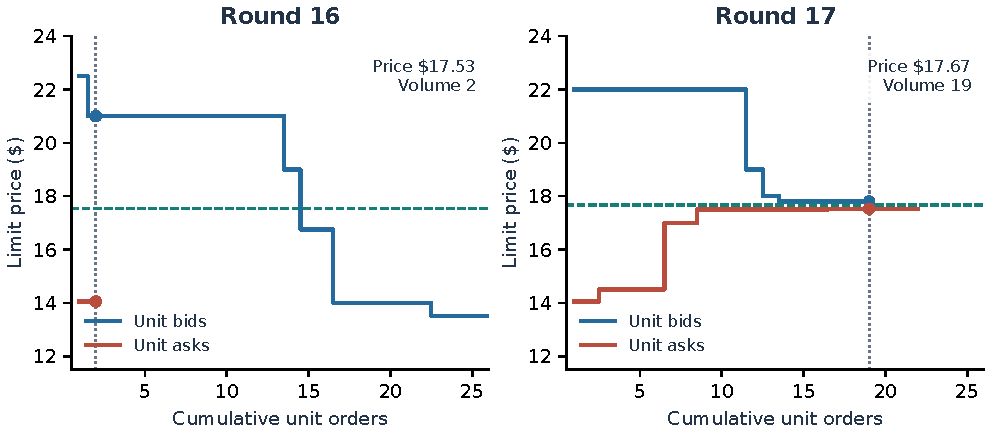
\includegraphics[width=\linewidth]{figures/clearing.pdf}
\caption{Admitted unit orders in the two trading rounds. Dots mark the marginal
matched bid and ask; vertical dotted lines mark traded quantity and horizontal
dashed lines mark the uniform clearing price. Only the first 26 units of each
book are displayed. Round 16 has just two units of supply.}
\label{fig:clearing}
\end{figure}

\Needspace{0.25\textheight}
\section{Workflow, pause rules, and EDSL execution}\label{app:execution}
\subsection{Observation policy as serialized predicates}
The following helper attaches checks to completed settlement steps. Two
consecutive non-null prices of at least \$17.50 cause a pause. Round 12 is
an observation checkpoint whose continuation is allowed only if the tape
contains no trades. Round 20 is another checkpoint. Resumption always requires
an explicit call; a pause does not redeem shares or erase future steps.

This is a retrospective encoding of the exploratory policy actually used.
The extension to 20 was declared after round 6 of the original run. It should
not be interpreted as a design fixed before that run began. The round-20
checkpoint also permits explicit continuation; it is not a terminal market state.
\WalkPause

\par\noindent
\begin{minipage}{\linewidth}
\subsection{Model and scripted executor assignment}
The execution plan binds trader work to EDSL's LLM executor with the pilot's
model settings. Exchange work uses a literal answer, which triggers the
already-declared settlement command without a model call.
\WalkPlan
\end{minipage}
\par

\subsection{Complete 30-round workflow and experiment bundle}
The builder places the market in persistent session scope. Each trader step
reads its private account and the public tape, then submits the structured
answer. Settlement waits for all assigned traders; the next order round waits
for settlement. The final \code{WorkflowExperiment} bundles the compiled
workflow, state definitions, agents, execution plan, and metadata.
\WalkBuild

\subsection{Save, load, and replay without experiment imports}
From the repository root, running the authoring file exports the specification
and the archived answers. It makes no model calls:
\begin{lstlisting}[language={},numbers=none]
python -m examples.asset_market.portable
\end{lstlisting}
Once exported, a process needs only the updated EDSL branch and JSON files:
\par\noindent
\begin{minipage}{\linewidth}
\begin{lstlisting}[numbers=none,breaklines=true]
import json
from pathlib import Path
from edsl.workflows import WorkflowExperiment

folder = Path("examples/asset_market/portable")
experiment = WorkflowExperiment.load(folder / "experiment.json")
answers = json.loads((folder / "responses.json").read_text())
output = "/private/tmp/asset-market-replay-new"
first = experiment.run(output, responses=answers)
# Paused after round 12: 144 decisions + 12 settlements.
second = experiment.run(output, responses=answers, resume=True)
# Paused after round 17: 204 decisions + 17 settlements.
\end{lstlisting}
\end{minipage}
\par
Supplying \code{responses} prohibits fallback to model calls; a missing
answer fails explicitly. A fresh-process acceptance test forbids every
\code{examples.*} import and checks the replayed accounts, tape, and order
log against the archive. All 48 shares remain live after round 17.

\subsection{Conducting a new model session}
For a new session, omit \code{responses} and choose a new output directory:
\begin{lstlisting}[numbers=none]
experiment = WorkflowExperiment.load(folder / "experiment.json")
first = experiment.run("new-market-session")
# If the round-12 continuation guard passes:
second = experiment.run("new-market-session", resume=True)
\end{lstlisting}
These calls use configured provider credentials and incur model charges.
The generic runner opens all ready work items before submitting answers,
pinning each trader's observations. Each round is one EDSL job: twelve agents
paired with twelve private scenarios using \code{zip\_assign}. EDSL runs the
interviews concurrently, and settlement waits for their accepted answers.
Pairings and frozen prompts are preserved in saved job specifications.
The sealed views and seeded tie priority preserve the saved-answer replay.
Fresh LLM decisions need not reproduce the historical prices.

Workflow and market state are persisted in SQLite, and live EDSL responses
are archived separately. Resumption verifies the entire pinned specification.
Idempotent submissions and recovery guard committed state effects against
duplication; they do not guarantee that a network retry never incurs another
provider request. No new hosted calls were made to produce this rewrite.

\clearpage
\section{Reproduction, audit, and archive repair}\label{app:reproduce}
\subsection{Executed commands and observation checkpoints}
These commands describe the two invocations used for this observation, run
from the repository root with the shared-state branch installed. They invoke
the EDSL Python API through the experiment driver; they are not generic
\code{ep run} CLI jobs. Re-executing them makes new paid model calls and need
not reproduce identical responses. The first command cannot overwrite an
existing run directory. Use the saved artifacts to reproduce this note.

\begin{lstlisting}[language={},numbers=none]
python -m examples.asset_market.run_gpt5_pilot \
  --stop-after 12 \
  --output examples/asset_market/runs/gpt5-short-pilot

python -m examples.asset_market.run_gpt5_pilot \
  --stop-after 20 --resume \
  --output examples/asset_market/runs/gpt5-short-pilot
\end{lstlisting}

At round 12, the checkpoint contained 144 trader responses, no transactions,
and a highest bid of \$20.50. The second invocation continued from the saved
accounts and histories; no earlier decision was regenerated. It stopped after
round 17, leaving 13 economic rounds unobserved. The stop condition, economic
horizon, and speculative prompts did not change during the extension.

\subsection{A Results-package export repair}
After the economic observation paused successfully, the second invocation
could not replace the existing round-12 \code{results.ep} package: EDSL's
default save operation protects an existing package. The durable market state,
workflow, and 204 raw responses were already present. The frozen executed
runner contains this original export call:
\begin{lstlisting}[numbers=none]
Results(survey=workflow.steps[0].survey, data=records).save(
    str(output / "results.ep")
)
\end{lstlisting}
Recovery reconstructed \code{records} from archived raw EDSL results for
completed work items and explicitly allowed a new Results commit. The
operational correction was:
\begin{lstlisting}[numbers=none]
Results(survey=workflow.steps[0].survey, data=records).save(
    str(output / "results.ep"), allow_new_commit=True
)
\end{lstlisting}
The earlier Results commit was retained and CSV exports were refreshed.
Recovery generated zero model calls and zero market commands. This correction
is documented separately rather than silently changing the source hash of the
executed runner. Future resumed exports need the same explicit save option;
changing frozen execution files would cause the existing run's hash check to
reject resumption.

\subsection{Audit evidence and artifact map}
The prefix audit reconstructs each account from its initial endowment and
private history. It checks signed fills, cash and inventory constraints,
interest and dividends, conservation under trading, total volume, every
private view, and the rendered prompt against that view. It also checks model
finish reasons, unique work-item coverage, Results row count, and the exact
source hashes pinned by the run. These are execution checks, not proof of
economically rational model behavior or fidelity to every source-paper detail.

\begin{center}\small
\begin{tabularx}{\linewidth}{@{}lX@{}}
\toprule
File(s) in the original run directory & Purpose \\
\midrule
\path{config.json} & Economic/model settings and four source SHA-256 hashes. \\
\path{workflow.json}, \path{execution-plan.json} & Full 30-round dependency definition and executor assignment. \\
\path{shared-state-definition.json} & Serializable machine, commands, and private view. \\
\path{workflow.sqlite} & Deliveries, answers, attempts, workflow events. \\
\path{shared-state.sqlite} & Market state and recorded reads/command effects. \\
\path{model-calls.jsonl}, \path{results.ep} & Raw EDSL calls and the versioned 204-row Results archive. \\
\path{summary.json}, \path{orders.json} & Round tape, accounts, and admitted orders. \\
\path{checkpoints/round-12/} & Observation checkpoint before extension. \\
\path{archive-recovery.json} & Record of the export-only recovery. \\
\bottomrule
\end{tabularx}\end{center}

The original run lives under
\path{examples/asset_market/runs/gpt5-short-pilot/}. The compact note bundle
includes all four fingerprinted source files, the self-contained native
authoring file and its equivalence-check record, the 204-decision and 17-round
CSV tables, configuration and audit summaries, the observation plan, an actual
prompt/answer example, and vector figures. Large SQLite histories and the full
raw-call archive remain in the original workspace; they are not duplicated
in the note bundle. Its \path{manifest.json} records hashes of the included
code, data, and figure files.

\subsection{Rebuilding the note without model calls}
From the repository root, the first command below audits the saved run and
regenerates its publication figures and source snapshots. The second compiles
the document. A recipient with only the note bundle can skip the Python step:
all figures, data, and listings needed for compilation are already present.

\begin{lstlisting}[language={},numbers=none]
python -m examples.asset_market.build_latex_note
cd examples/asset_market/latex-note
latexmk -pdf -interaction=nonstopmode -halt-on-error note.tex
\end{lstlisting}

For inference beyond this exploratory observation, the next experiment would
need a fixed observation policy, repeated independent sessions, matched model
and prompt comparisons, and enough rounds to observe both price formation and
any subsequent reversal. This note reports only the saved 17-round prefix.

\end{document}
